\subsection{Action Detection}
\label{sec:action_detection}
From the description of a query, we can obtain multiple actions of a vehicle of interest, such as \textit{``go straight''}, \textit{``stop''}, \textit{``turn right''}, \textit{``turn left''}, and so forth. In this section, we present our method to detect two important action types: stop and turn (left or right). Our method analyzes the trajectory of a vehicle, a sequence of points $p_1$, $p_2$, ..., $p_n$, where $p_i$ is the center of the vehicle's bounding box at the $i^{th}$ frame.
\subsubsection{Stop Detection}
To detect a stop event, we first calculate a sequence of motion speed $v_i$ = $dist(p_{i+k}, p_i)$ where $dist$ is the Euclidean distance and $k = 5$ in our implementation. To remove noise of a temporary slow down in speed, we apply a moving average filter with the window size $delta = 10$ on the sequence of $v_i$. We consider a stop event occurs when the speed is significant small, comparing to the average speed. We choose a simple yet efficient formula to detect a stop event if the motion speed $v_i < \alpha \times mean\{v_i\}$ where $\alpha = 0.15$.

\subsubsection{Turn Detection}
\begin{figure}[!htb]
    \centering
    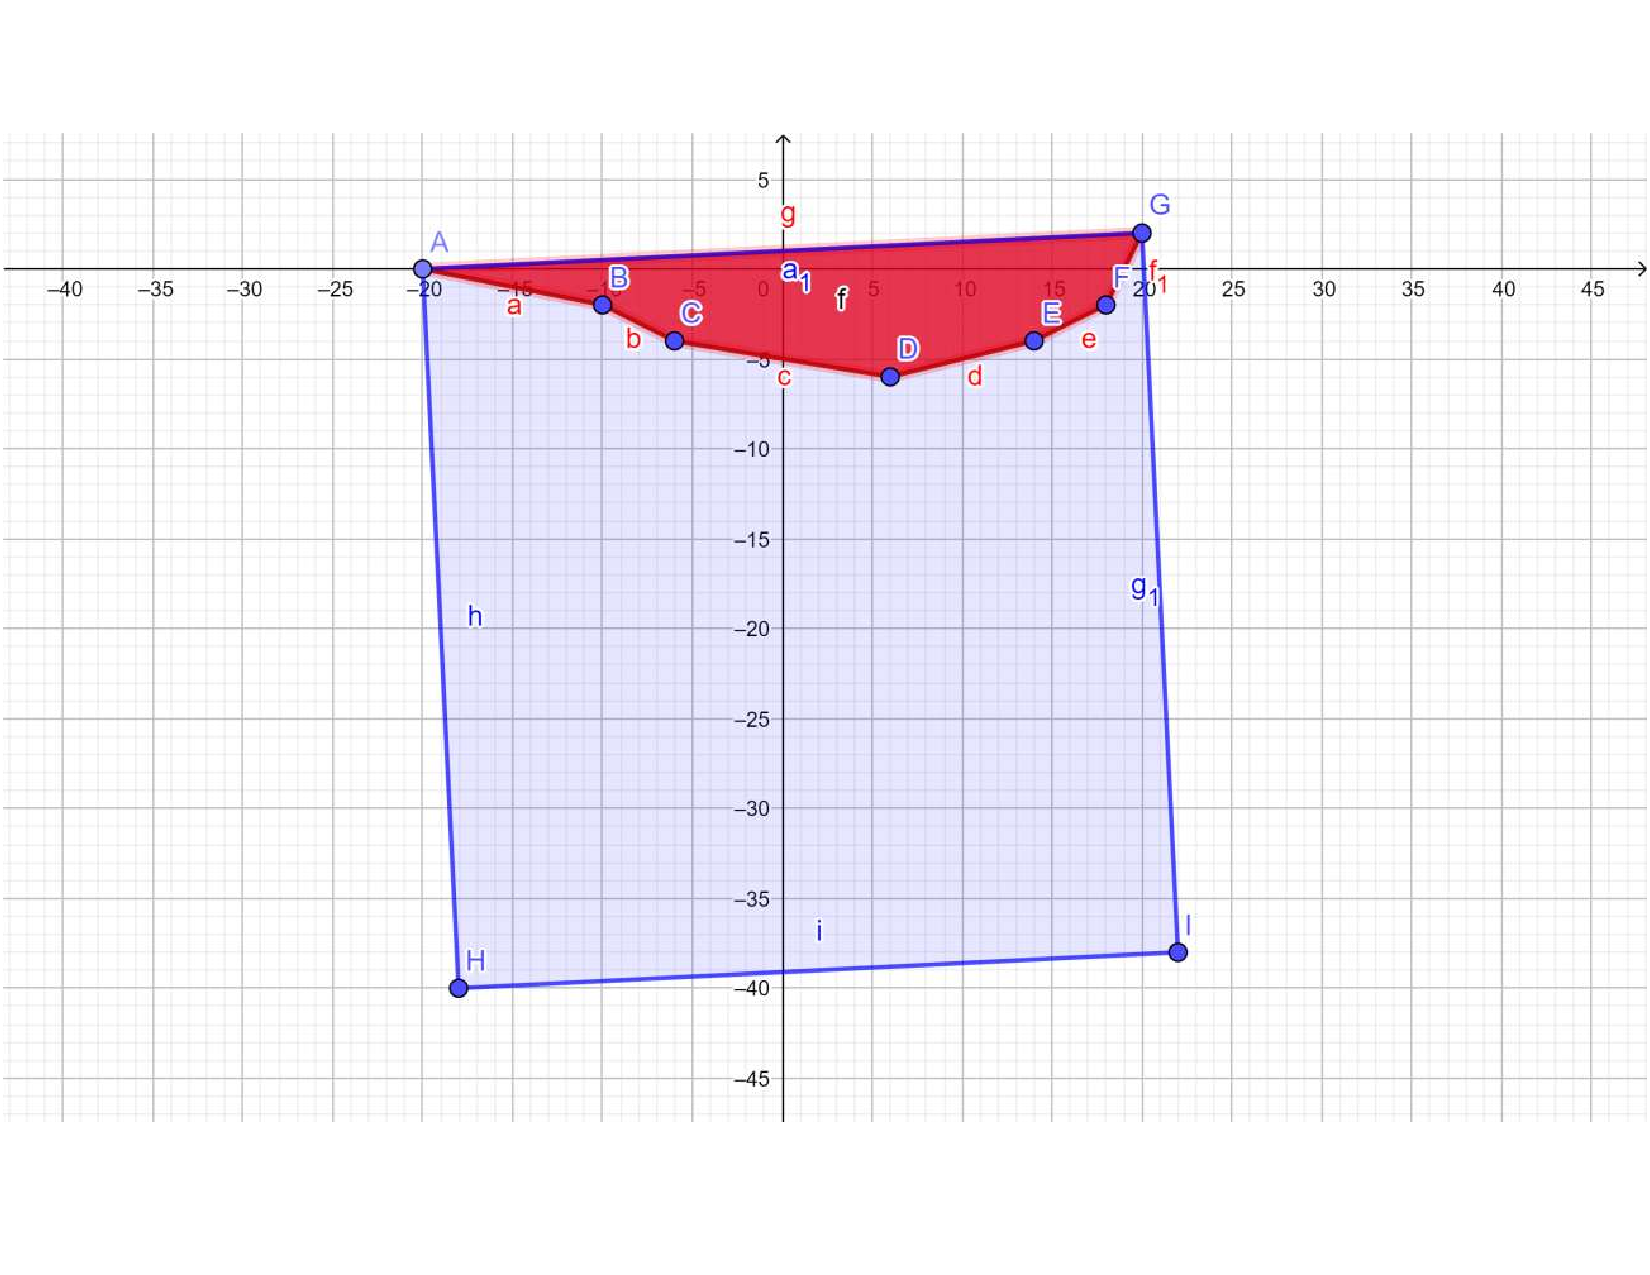
\includegraphics[width=\linewidth]{images/methods/SignedArea_foxit.pdf}
    \caption{Illustration for using algebraic area to evaluate the direction of a motion trajectory.}
    \label{fig:signed_area}
\end{figure}
We use algebraic area to classify the motion direction of a vehicle's trajectory into 3 categories:  \emph{``go straight''},  \emph{``turn right''}, and \emph{``turn left''}. 
Let $A$ be the algebraic area corresponding to the polygon with $n$ vertices $p_1$, $p_2$, ..., $p_n$. 
\[
A = \frac{{\sum\nolimits_{i = 3}^n {\overrightarrow {p_1 p_{i - 1} }  \times \overrightarrow {p_1 p_i } } }}{2}
\]

The vehicle is going in a straight line if $|A|$ is small. If $|A|$ is considerably large, the vehicle is like to turn left or right. The vehicle turns left when $A > 0$, and turns right when $A < 0$.
We observe that the error due to possible distortion in cameras is directly proportional to the square value of the distance between the start and end points in the trajectory $|p_1p_n|^2$.
We define $B = A/|p_1p_n|^2$. As illustrated in Figure \ref{fig:signed_area}, $B$ is the (signed) ratio between the area of the red polygon and the blue square. If $|B|$ is greater than a certain threshold $\epsilon$, we conclude that the vehicle turns (left or right), and goes straight otherwise.
